\documentclass[journal]{IEEEtran}
\usepackage{tikz}
\usepackage{cite}
\usetikzlibrary{decorations.pathreplacing,angles,quotes}

% correct bad hyphenation here
\hyphenation{op-tical net-works semi-conduc-tor}

\begin{document}
%
% paper title
\title{Project Report}

% puts info about authors at bottom of first page
\author{Lawrence~Owusu,~Jordan~Sturtz,~and~Swetha~Chittam~% <-this % stops a space
  \thanks{The authors are graduate students at NCA\&T}% <-this % stops a space
}

% note the % following the last \IEEEmembership and also \thanks -
% these prevent an unwanted space from occurring between the last author name
% and the end of the author line. i.e., if you had this:
% \author{....lastname \thanks{...} \thanks{...} }
%                     ^------------^------------^----Do not want these spaces!

% The paper headers
% The only time the second header will appear is for the odd numbered pages
% after the title page when using the twoside option.
\markboth{CS851 - Deep Learning: Project Report}%
{Shell \MakeLowercase{\textit{et al.}}: CS851 - Deep Learning: Project Report}

% make the title area
\maketitle

% As a general rule, do not put math, special symbols or citations
% in the abstract or keywords.
\begin{abstract}
  De novo protein sequencing using mass spectrometry or Edman degradation
  suffers from the problem of producing only partial sequences of target proteins.
  We explore the possibility of using deep learning techniques to perform the 
  task of predicting gaps in partially sequenced proteins. Our method involves
  querying the NCBI Protein Blast server for closest matching homologous sequences
  to a partial sequence, then training two deep learning models to predict
  in the forward and reverse directions the missing gaps. Our results show
  high accuracy (98-99\%) in filling gaps of a particular partially sequenced 
  de novo sequence of the light chain of alemtuzumab.

\end{abstract}

% Note that keywords are not normally used for peerreview papers.
% \begin{IEEEkeywords}
% IEEE, IEEEtran, journal, \LaTeX, paper, template.
% \end{IEEEkeywords}

% For peer review papers, you can put extra information on the cover
% page as needed:
% \ifCLASSOPTIONpeerreview
% \begin{center} \bfseries EDICS Category: 3-BBND \end{center}
% \fi

%
% For peerreview papers, this IEEEtran command inserts a page break and
% creates the second title. It will be ignored for other modes.
\IEEEpeerreviewmaketitle

\section{Introduction}
  \IEEEPARstart{P}{rotein} structure sequencing remains one of the challenges in the field of computational biology.
    Determination of accurate protein structure is important in developing deep understanding of the
    functions of proteins and their applications of drug and inhibitor discovery and design.

    Protein sequencing begins in the lab using techniques such as mass spectrometry or Edman degradation
    to identify partial sequences of proteins \cite{mann2016rise, edman1949method}. Various techniques exist for using these
    partial sequences to construct the full protein sequence
    \cite{standing2003peptide,perkins1999probability, eng1994approach, yang2021full}.

    In our paper, we develop an approach using deep learning techniques to predict missing gaps in peptide sequences.
    Our approach begins with a partial sequence with gaps of known size. To retrieve the relevant training data,
    we query the National Center For Biotechnology Information (NCBI) Protein Blast server to retrieve the highest matching
    homologous sequences to our partial sequence \cite{ncbi}.We then train and deploy two models: one to learn dependencies
    in the forward direction and another to learn dependencies in the reverse direction. We combine the two 
    models' predictions to fill the gaps in the de novo protein sequence.

    We train and evaluate four competing hybrid deep learning models combining LSTM and CNN layers.     
    For the purpose of this project, we tested our model against only a single 
    target sequence: the light chain of alemtuzumab. Our results show high accuracies (98-99\%) for all four of our model architectures,
    with our Bi-LSTM-CNN model outperforming the others at 99.04\%.

    \subsection{Related Work}

    Mass spectrometry continues to be a dominant method to perform protein sequencing \cite{mann2016rise}.
    In this approach, multiple proteases are employed to cleave the same protein sample separately.
    Because the cleavage of protein by the protease generates overlapping peptides, merging the spectral
    pairs of the overlapping peptides consecutively assembles into long contigs from which de novo
    sequences are obtained \cite{liu2014novo}.

    Some researchers on protein sequencing problems focus on identifying proteins or generating full protein sequences
    by comparing partial sequences to known protein databases to infer the missing gaps in mass spectral data
    \cite{eng1994approach, perkins1999probability}. Others focus on developing techniques for de novo protein sequencing,
    which refers to the process of sequencing proteins without the use of a protein database or with minimal use of
    genomic data \cite{standing2003peptide, bandeira2008automated}.

    Over the last 10 years, de novo protein sequencing has been researched
    extensively in computational proteomics and have been used successfully to deduce peptide sequence
    of un-sequenced organisms, antibodies and post-translationally modified peptides
    \cite{ma2012novo,veltman2012novo, bandeira2007spectral}. For example,
    Mai et al. reported that their assembling algorithm, Multiple Contigs and Scaffolding
    successfully assembles the de novo identified peptides in contig-scaffold fashion, resulting in
    100\% coverage and 98.69-100\% accuracy on three proteins and replications. The Multiple Contigs
    and Scaffolding algorithm has provided robust and accurate software for full-length protein sequencing
    after de novo identification of peptides \cite{mai2022highly}

    Similarly, Yang et al. reported 100\% accuracy for full-length de novo sequencing
    for light chains of Herceptin and bovine serum albumin (BSA) when their proposed method was applied to de novo
    sequencing of bovine serum albumin (BSA) and monoclonal antibody Herceptin. However, the accuracy marginally dropped to
    99.7\% for the heavy chains of Herceptin \cite{yang2021full}.

    Protein sequencing is only one type of sequencing problem in biology. Related types of sequencing problems include
    single-cell protein sequencing or whole genomic sequencing \cite{wang2015advances,pareek2011sequencing}.

\section{Method}

  \subsection{Data Collection}
    For our initial project, we used as a target sequence the light chain of alemtuzumab referenced in Liu, et al.
    \cite{liu2014novo}. We manually removed the gaps produced by Liu et al.'s tandem mass spectrometry approach, then
    entered that sequence into NCBI's Protein Blast Server to retrieve the closest matching homologous sequences \cite{ncbi}.
    We used the top ten homologous sequences as training data. The closest matching homologous sequences in our training
    data range from 89.32\% to 82.52\% similarity.

  \subsection{Data Preprocessing}
    We generated from our homologous sequences all kmers. A kmer is a any substring of length K. For our models, we chose a
    kmer-length of 5. Each kmer represents a single input, and the output of each associated kmer is the next character in the sequence.
    Thus, for instance, if one of our homologous sequences contains the substring "DIQMSQ", then a single training instance would be
    the input-output tuple (DIQMS, Q).

    From our ten homologous sequences, we generated 2106 number of input-output pairs with an input length of 5.
    The kmer length represents the timesteps in our LSTM layer.
    To be fed into a neural network, the data must be encoded numerically, so we assigned integer labels to each character.
    The output of each training instance is a
    one-hot encoded vector to represent the target classes. Since we are training two models, one for forward prediction
    and one for reverse prediction, we generate the same training data in both the reverse and forward directions.

    The samples of forward and reverse input-output pairs are divided into training and validation sets with the ratio of
    90\% and 10\% respectively. The validation set is used to prevent overfitting.

\subsection{Data Normalization}
    The input pairs are normalized by dividing with number of classes to obtain a range between [0, 1].
    The number of classes are determined by extracting all the unique characters from the input sequences.
    This data normalization technique is applied to forward, reverse and test data input-output pairs.
    Normalization helps speed the training process.

\subsection{Model Selection}

    For our sequence prediction task, we built four deep learning models combining convolutional neural
    networks (CNN) with long short term memory (LSTM). The CNN layer in theory helps with automatic feature extraction, in particular
    if there are patterns within each kmer that can be extracted for better predictions. The LSTM layer is the 
    core of our models, since LSTM is useful for learning sequence dependencies in our input data.
    For our four hybrid models, we also added two dense hidden layers with ReLu activation and a
    final output layer with softmax activation.

    It is not clear a priori whether LSTM or Bi-LSTM would be more effective in our prediction task; nor is it clear
    whether the addition of the convolutional layer would improve our results. We thus opted to evaluate and compare
    four hybrid models: LSTM, CNN-LSTM, Bi-LSTM, and CNN-Bi-LSTM.
    The workflow for the proposed approach is shown in Figure~\ref{fig:model_diagram}.

    \begin{figure}[h]
      \centering
      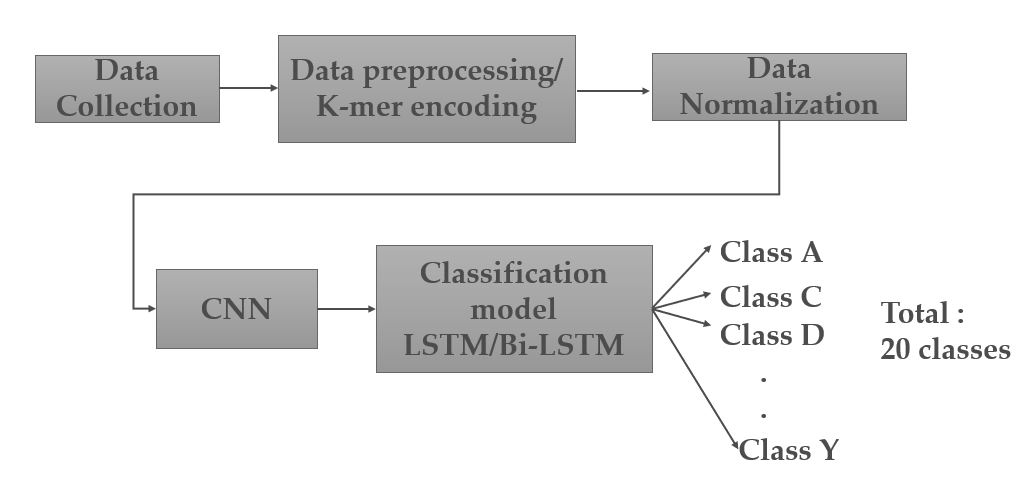
\includegraphics[width=8cm]{figures/Model_Diagram.JPG}
      \caption{Model Diagram for Multi-Classification of Sequence Data}
      \label{fig:model_diagram}
    \end{figure}

    \subsubsection{CNN}
      CNN is a powerful deep learning technique for feature extraction.
      CNN is often used on 2-dimensional and 3-dimensional datasets, e.g. image or video datasets.
      We use a 1-dimensional convolutional layer that convolves the kmers to extract any meaningful
      features. The convolutional layer has 128 filters with a kernel size of 3, so minimally the kmer-length cannot be
      smaller than 3. The feature maps from this layer forms as input to the LSTM or Bi-LSTM layer.

    \subsubsection{LSTM}
      The LSTM architecture consists of a set of chained together cells called "memory blocks". The number
      of memory blocks in the chain equals the length of the timesteps in our target dataset.
      Each memory cell has three gating units (forget, input, and output gates) which
      conditionally regulate how information flows into and out of the memory block (Figure~\ref{fig:lstm_architecture}). 
      Intuitively, the "forget" gate can be viewed as a step where irrelevant information from the hidden state
      is first "forgotten" before being passed to the input gate, which constructs the new cell state.
      Before that cell state can output its value to the next memory cell, it is filtered again through
      an output gate that decides what values to keep internal to the memory cell (i.e. the hidden state)
      and what to output to the next memory cell or final output layer.
      The LSTM layer is helpful, therefore, for learning the important sequence dependencies for performing
      sequence predictions.

      \begin{figure}[h]
        \centering
        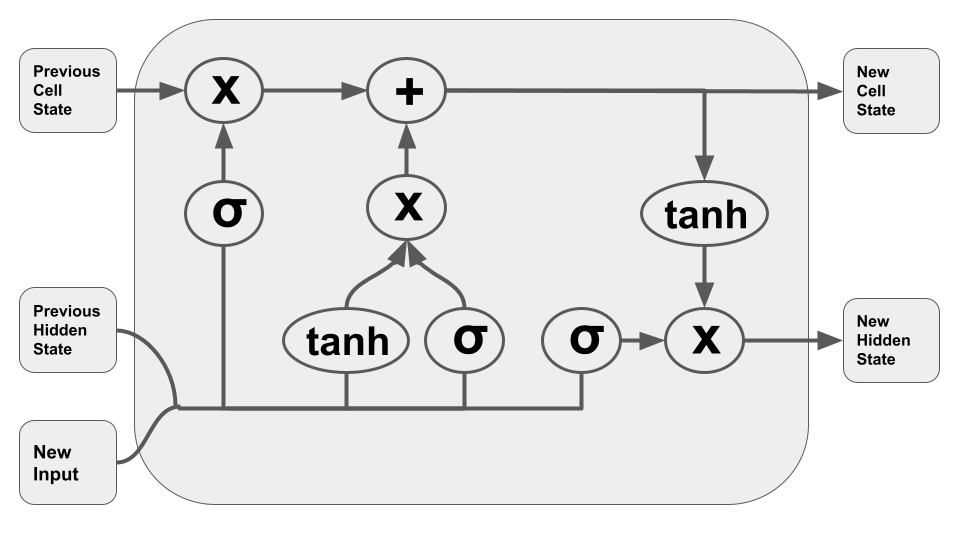
\includegraphics[width=8cm]{figures/jordan_lstm_architecture.png}
        \caption{LSTM Architecture Inside a Memory Cell}
        \label{fig:lstm_architecture}
      \end{figure}

    \subsubsection{Bi-LSTM}
      Bidirectional LSTM (Bi-LSTM) is a modification of the LSTM architecture that permits the model to learn both the
      forward and reverse dependencies. Bi-LSTM uses two LSTM layers, one consuming
      the timesteps in the forward direction and the other consuming the timesteps in the reverse direction.
      The two layers then merge their results to produce the final output. See Figure~\ref{fig:bidirectional_diagram}
      for an illustration.

      \begin{figure}[h]
        \centering
        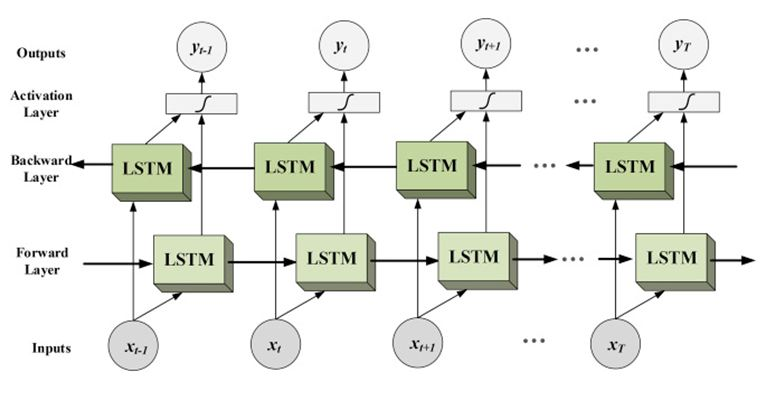
\includegraphics[width=8cm]{figures/bidirectional-lstm.jpeg}
        \caption{Bidirectional LSTM Architecture}
        \label{fig:bidirectional_diagram}
      \end{figure}

\section{Overall Model Architecture}

  All four of our hybrid models share common features. If there is a convolutional
  layer, it is the first layer after the input layer. After that,
  the next layer is either the LSTM or Bi-LSTM layer. After that,
  the results are passed to two hidden densely connected layer with ReLu activation,
  which pass their results to the final dense layer with
  softmax activation. The number of neurons in the final output layer
  equals the number of our target classes. See Figure~\ref{fig:model_architectures}.

  \begin{figure}[h]
    \centering
    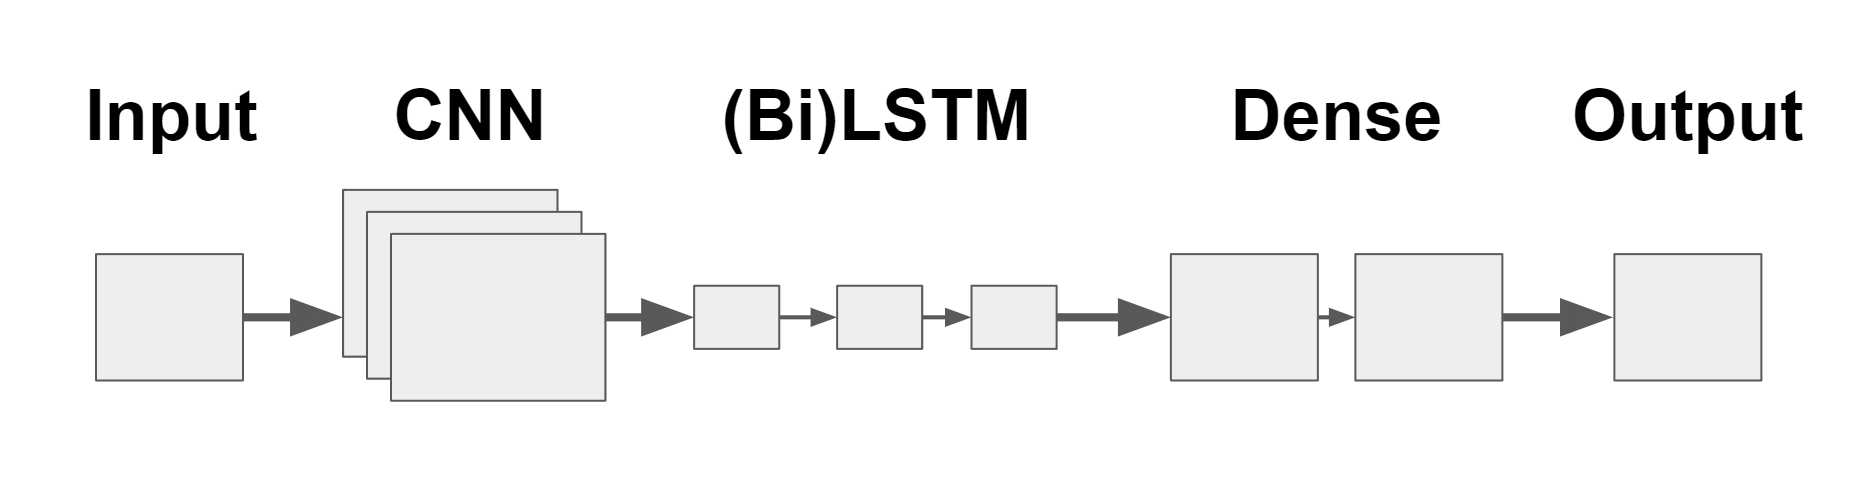
\includegraphics[width=8cm]{figures/model_architectures.png}
    \caption{Deep Learning Model Architecture}
    \label{fig:model_architectures}
  \end{figure}

\section{Experimental Results}
  \subsection{Experimental Model Architectures}

    We initially experimented with a simple input-LSTM-output architecture. By itself, a single LSTM layer acheived high
    accuracy with minimal amount of training. We attribute this largely to the quality of our
    training dataset. Indeed, all of the training instances had between 89.32\% to 82.52\% similarity
    match to our target sequence. The lower the similarity between our target sequence and the training
    data, the lower our expected accuracy and thus the greater the difficulty in the sequencing task.

    We added two hidden Dense layers after the initial LSTM layer and the accuracy improved marginally.
    In subsequent model trials, we kept the two hidden layers since they showed marginal improvement
    over leaving them out.

    We settled on four competing architectures to run: LSTM, CNN-LSTM, BiLSTM, and CNN-BiLSTM.
    Their testing accuracies, final loss values, and final validation loss values are displayed
    in Table~\ref{tab:model_results}.

    Our models all exhibited slight overfitting, though not enough to be significant.
    Figures~\ref{fig:lstm_accuracy},~\ref{fig:cnn_accuracy},~\ref{fig:bilstm_accuracy},~and~\ref{fig:cnn_bilstm_accuracy}
    plot training accuracy against validation accuracy for our four models, and 
    Figures~\ref{fig:lstm_loss},~\ref{fig:cnn_loss},~\ref{fig:bilstm_loss},~and~\ref{fig:cnn_bilstm_loss}
    plot training loss versus validation loss for all four models.

    \begin{table}[h!]
      \begin{center}
        \begin{tabular}{l|l|l|l} % <-- Alignments: 1st column left, 2nd middle and 3rd right, with vertical lines in between
          & \textbf{Test Accuracy} & \textbf{Training Loss} & \textbf{Validation Loss}\\
          \hline
          LSTM        & $98.56\%$ & $0.0964$ & $0.4546$ \\
          Bi-LSTM     & $98.09\%$ & $0.1282$ & $0.6051$ \\
          CNN-LSTM    & $98.56\%$ & $0.0948$ & $0.5604$ \\
          Bi-CNN-LSTM & $99.04\%$ & $0.0884$ & $0.6719$ \\
        \end{tabular}
        \caption{Comparing Different Model Architectures}
        \label{tab:model_results}
      \end{center}
    \end{table}
  
    \begin{figure}[h]
      \centering
      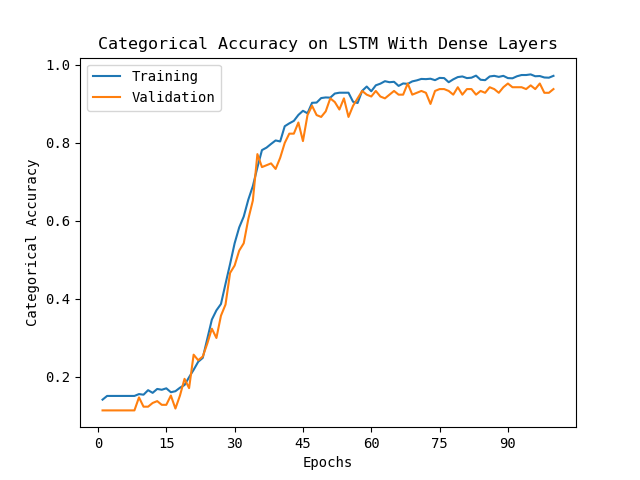
\includegraphics[width=8cm]{figures/01-58-36Forward_LSTM With Dense Layers_accuracy.png}
      \caption{LSTM Accuracy}
      \label{fig:lstm_accuracy}
    \end{figure}

    \begin{figure}[h]
      \centering
      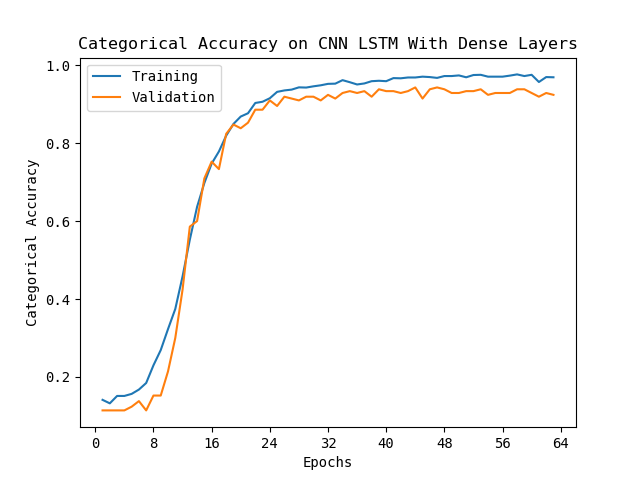
\includegraphics[width=8cm]{figures/02-07-24Forward_CNN LSTM With Dense Layers_accuracy.png}
      \caption{CNN LSTM Accuracy}
      \label{fig:cnn_accuracy}
    \end{figure}

    \begin{figure}[h]
      \centering
      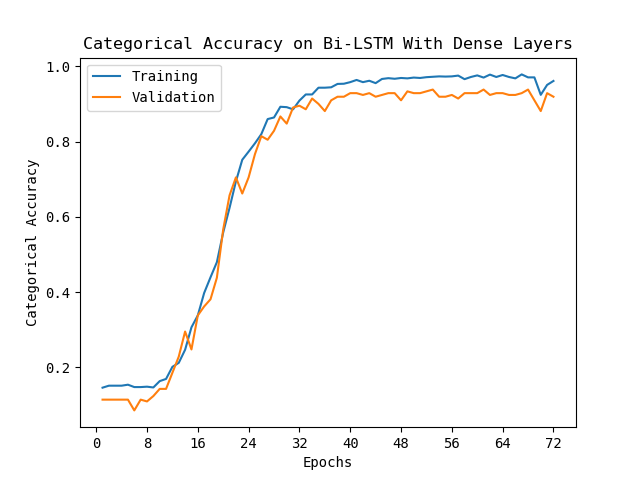
\includegraphics[width=8cm]{figures/02-31-57Forward_Bi-LSTM With Dense Layers_accuracy.png}
      \caption{Bi-LSTM Accuracy}
      \label{fig:bilstm_accuracy}
    \end{figure}

    \begin{figure}[h]
      \centering
      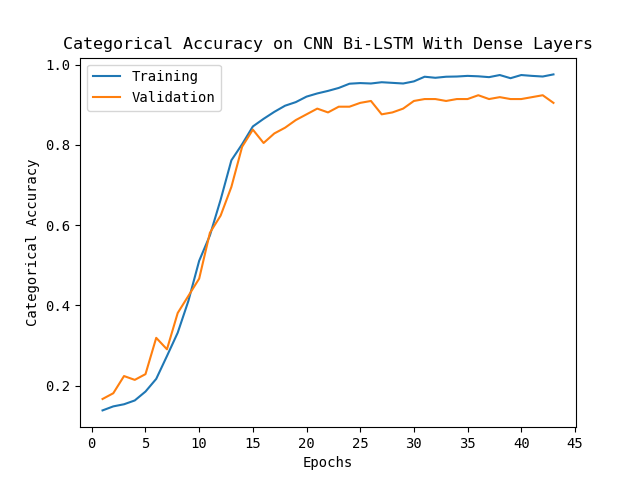
\includegraphics[width=8cm]{figures/02-34-46Forward_CNN Bi-LSTM With Dense Layers_accuracy.png}
      \caption{CNN Bi-LSTM Accuracy}
      \label{fig:cnn_bilstm_accuracy}
    \end{figure}

    \begin{figure}[h]
      \centering
      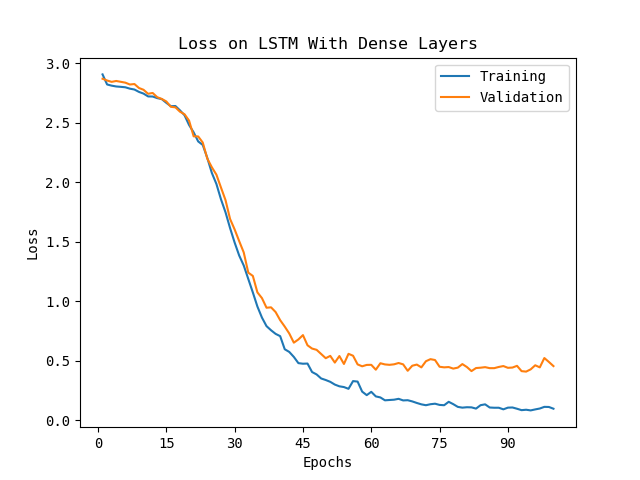
\includegraphics[width=8cm]{figures/01-58-36ForwardLSTM With Dense Layers_loss.png}
      \caption{LSTM Loss}
      \label{fig:lstm_loss}
    \end{figure}

    \begin{figure}[h]
      \centering
      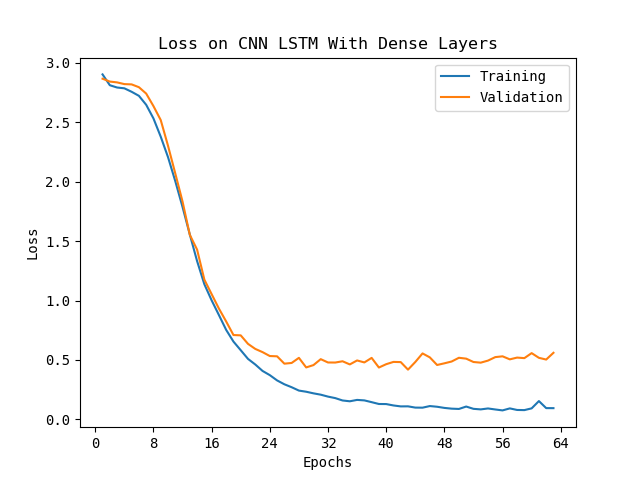
\includegraphics[width=8cm]{figures/02-07-24ForwardCNN LSTM With Dense Layers_loss.png}
      \caption{CNN LSTM Loss}
      \label{fig:cnn_loss}
    \end{figure}

    \begin{figure}[h]
      \centering
      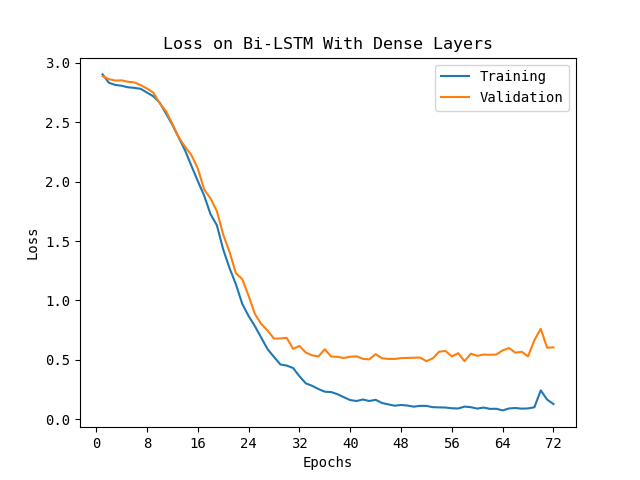
\includegraphics[width=8cm]{figures/02-31-57Forward_Bi-LSTM With Dense Layers_loss.png}
      \caption{Bi-LSTM Loss}
      \label{fig:bilstm_loss}
    \end{figure}

    \begin{figure}[h]
      \centering
      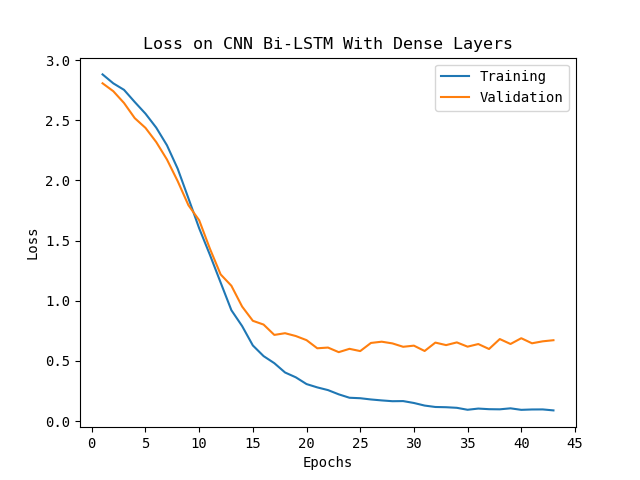
\includegraphics[width=8cm]{figures/02-34-46Forward_CNN Bi-LSTM With Dense Layers_loss.png}
      \caption{CNN Bi-LSTM Loss}
      \label{fig:cnn_bilstm_loss}
    \end{figure}

  \subsection{Hyperparameters}

    Our hyperparameters were chosen through manual trial-and-error. We did not implement
    any regularization techniques, nor did we use our validation set or cross validation to tune 
    any hyperparameters. All of our results for our different model architectures were generating
    high accuracy (98-99\%) on our single de novo sequence. Table~\ref{tab:hyperparameters}
    displays our chosen hyperparameters.

    \begin{table}[h!]
      \begin{center}
        \caption{Hyperparameters}
        \label{tab:hyperparameters}
        \begin{tabular}{l|l|l} % <-- Alignments: 1st column left, 2nd middle and 3rd right, with vertical lines in between
          & \textbf{Hyperparameter} & \textbf{Value} \\
          \hline
          \textbf{Shared} & Kmer Length                      & 5 \\
                          & Epochs                           & 100 \\
                          & First Dense Layer Neurons        & 128 \\
                          & Second Dense Layer Neurons       & 64 \\
                          & Cost Function                    & Categorical Cross Entropy \\
                          & Optimizer                        & ADAM \\
                          & Output Activation Function       & Softmax \\
                          & Dense Layer Activation Function  & ReLu \\
                          & Batch Size                       & 64 \\
          \hline
          \textbf{CNN}    & Number of Convolutional Filters  & 128 \\
                          & Convolutional Filter Size        & 3 \\
          \hline
          \textbf{LSTM}   & Number of LSTM Neurons           & 256 \\
        \end{tabular}
      \end{center}
    \end{table}

  \subsection{Predictions on De Novo Sequence}
    To deploy our models to predict gaps in our de novo sequence, 
    we trained two models: one to learn the dependencies in the forward direction and
    one to learn the dependencies in the reverse direction. This was necessary to predict 
    gaps in the beginning or end of the target sequence. 
    For example, if our target sequence begins with "DIQMSP" and we want to predict "DIQ", then
    we cannot predict from the forward direction, since "DIQ" is the absolute start of 
    the sequence. We must therefore be able to predict "DIQ" given the sequence
    ahead of it. Similarly, we must predict in the forward direction for gaps at the absolute end of the sequence.

    This use of two models implies a potential disagreement: one model may predict
    a different value than the other for those middle gaps with enough
    preceding values to create a valid input. See Figure~\ref{fig:forward_reverse_predictions}
    for an example of two different predictions from one sample run.
    
    To resolve any disagreement between the two models, 
    we opted to choose the prediction with the highest corresponding associated
    probability. By associated probability, we mean the output value
    of the output class with the highest probability.
    Since softmax outputs a probability distribution over the target classes,
    the prediction with the higher associated probability ought to be 
    preferred since its higher probability represents the "certainty"
    the model has in its prediction. 

    With this simple algorithm, we deployed our dual models to predict
    gaps in our de novo sequence, achieving 100\% accuracy for the test gaps.
    See Figure~\ref{fig:full_predictions}.

    \begin{figure}[h]
      \centering
      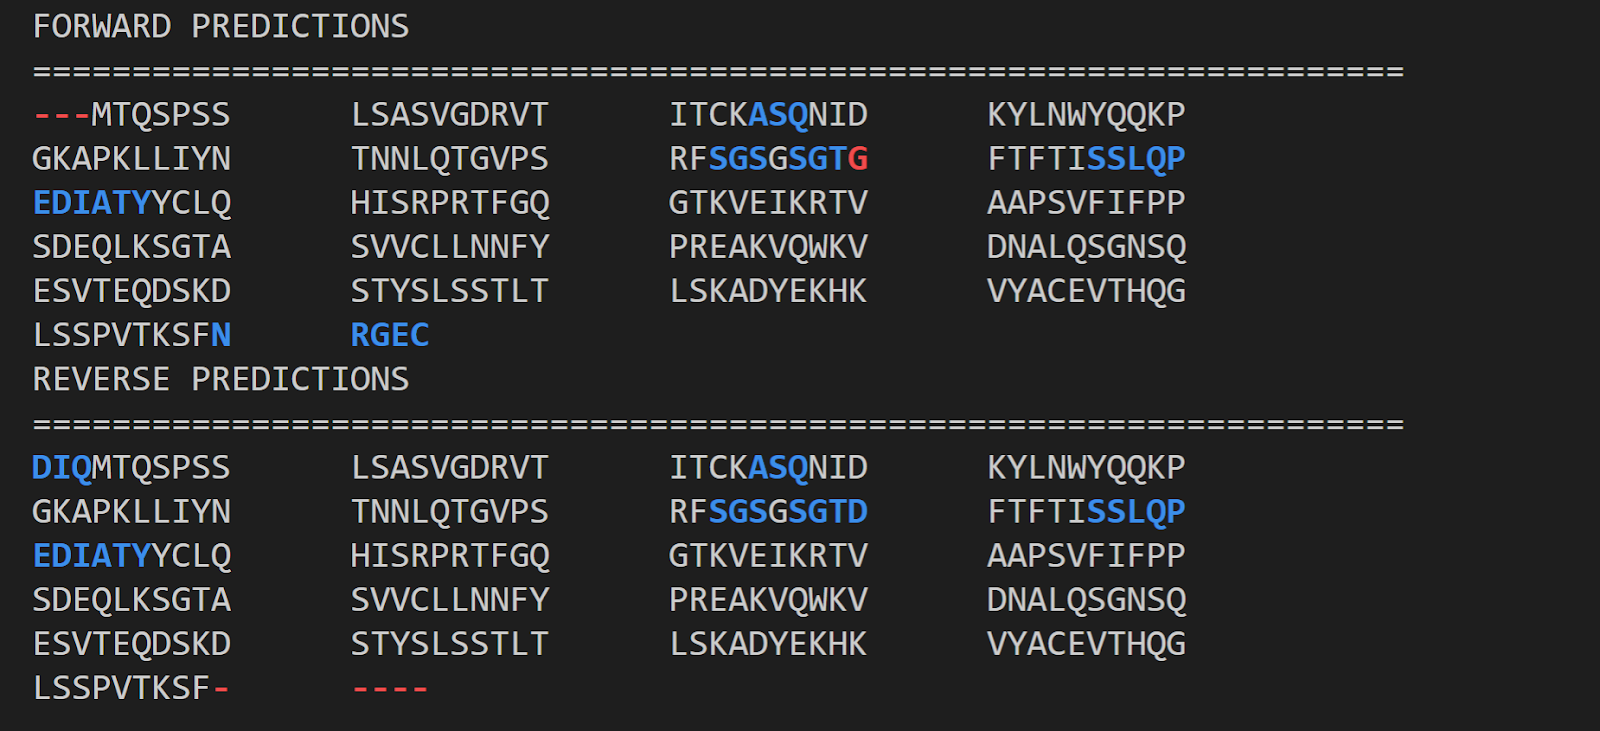
\includegraphics[width=8cm]{figures/forward_reverse_predictions.png}
      \caption{Illustration of Conflicting Predictions}
      \label{fig:forward_reverse_predictions}
    \end{figure}

    \begin{figure}[h]
      \centering
      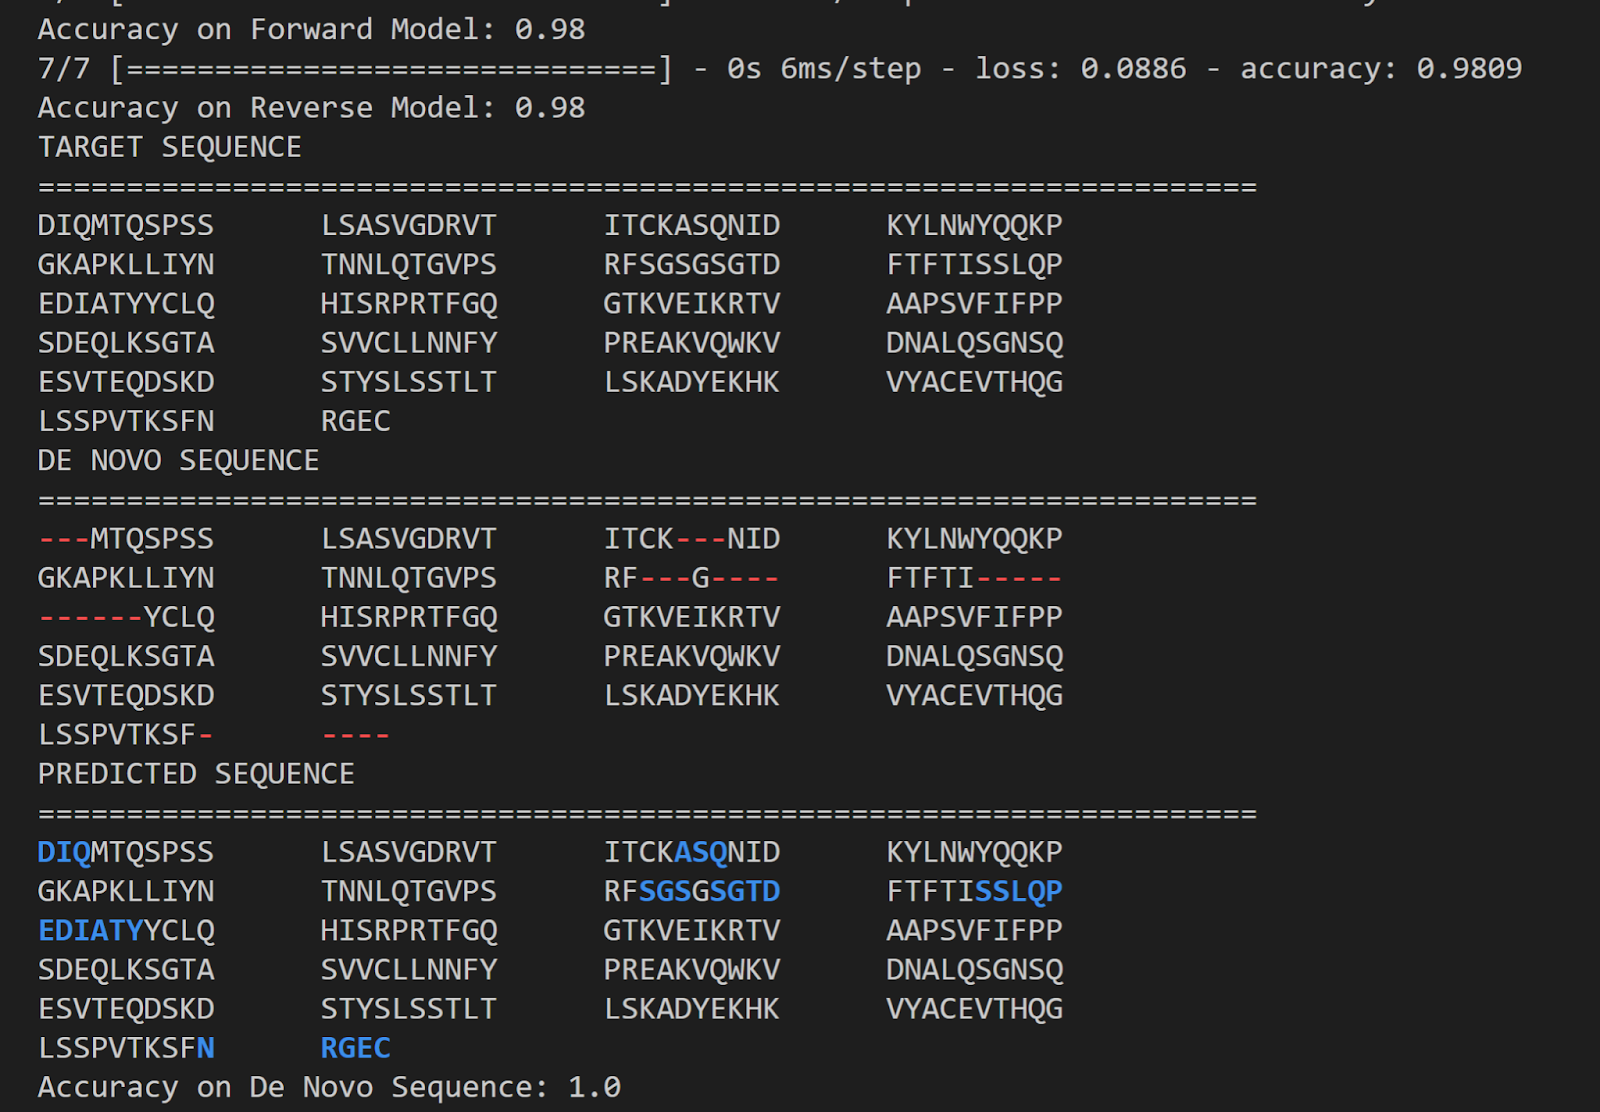
\includegraphics[width=8cm]{figures/full_predictions.png}
      \caption{Illustration of Complete Predictions}
      \label{fig:full_predictions}
    \end{figure}

\section{Conclusion}
  Our project aims to explore the possibility of using deep learning techniques to 
  solve an otherwise hard problem of predicting gaps in partial peptide de novo 
  sequences. We have demonstrated that with various LSTM-based deep learning models
  it is possible to achieve high accuracy on peptide sequences with gaps that have high 
  similarity scores in known protein databases.

  The approach we describe here generalizes to any other de novo sequence and in fact
  other sequencing problems beyond protein sequencing. Further research is needed to 
  explore the challenges and limitations of this approach, in particular for
  de novo sequences for which the highest similarity score in known protein databases 
  is comparatively low. Moreover, our approach relies on an assumption that gap 
  lengths in partial sequences are known in advance. In practice, partial sequence
  gaps may be unknown. It may be possible to solve this problem by employing
  forward and reverse predictions to generate overlapping sections or to use other 
  data features (for instance, known total mass of the gap) to successfully predict
  gaps of unknown length.

\bibliographystyle{IEEEtran}
\bibliography{main}

\end{document}
